\documentclass[a4paper,11pt]{article}
\usepackage[utf8]{inputenc}
\usepackage{tikz}
\usetikzlibrary{shapes}

\thispagestyle{empty} % no pagenumber. The form should be a stand alone macro... later.

\definecolor{SEPAOrange}{RGB}{254,213,161}
\definecolor{SEPADOrange}{RGB}{253,185,19}
\definecolor{SEPABlindcolor}{RGB}{255,0,0}


\begin{document}

SEPA-Überweisung

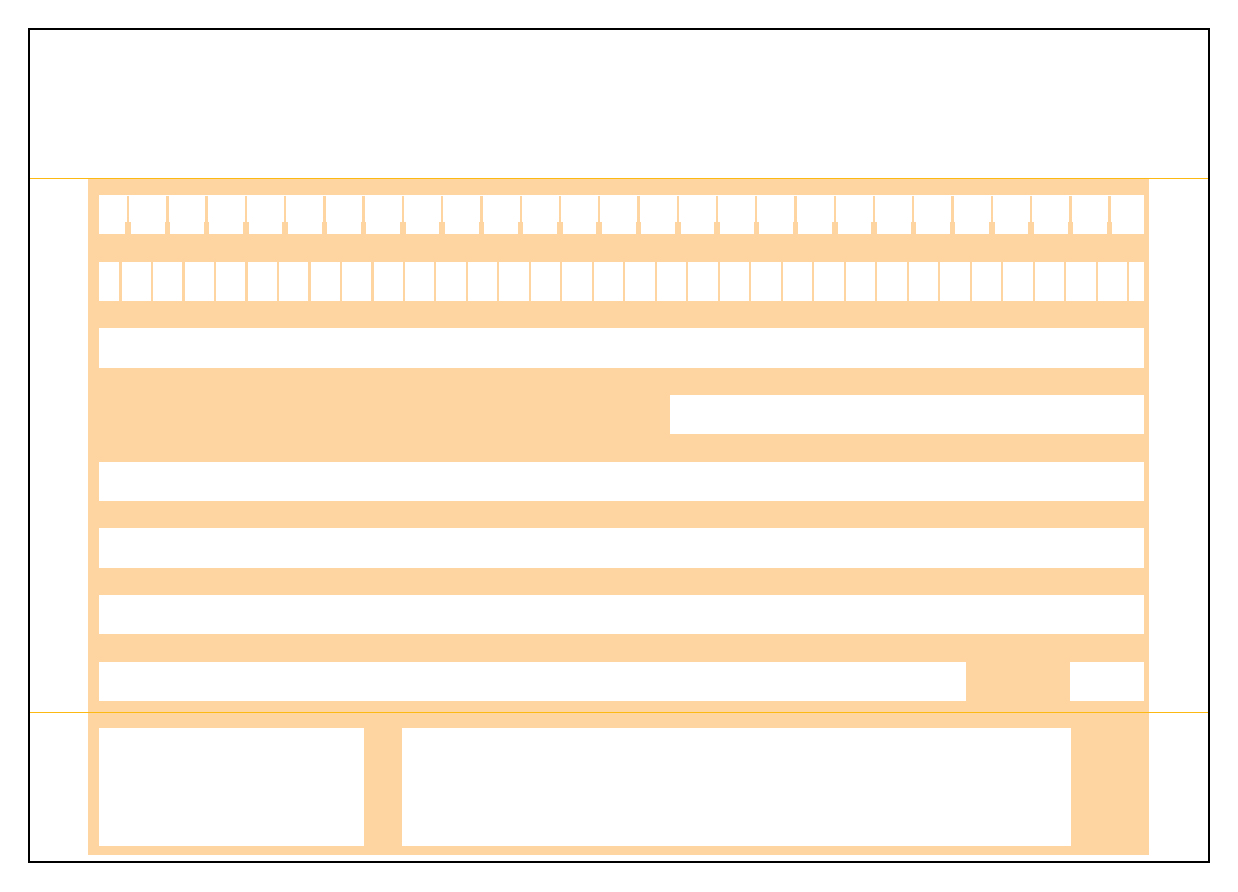
\begin{tikzpicture}[x=1 mm, y=-1mm]
\pgfmathsetmacro{\yh}{4.2333} % y heigth step defined as 1/6 inch =>  1/6 * 25.4 mm = 4.2333 mm
\pgfmathsetmacro{\xs}{9} % x start (own definition)
\pgfmathsetmacro{\xe}{141.5} % x end (own definition)
\pgfmathsetmacro{\widefield}{4.9859} % def: 134.62 mm / 27
\pgfmathsetmacro{\narrowfiels}{3.9594} % def: 134.62 mm/ 34

\filldraw[draw=black,color=SEPAOrange] (7.62, 4.5*\yh) rectangle (149.86-7.62,105.83-1); %orange background

\filldraw[draw=black,color=white] (\xs, 5*\yh) rectangle (\xe, 6.5*\yh -1.5); %Recepient 27 Char
\foreach \x in {1,...,26}
{
 \draw[color=SEPAOrange, line width=0.3mm] (7.62 + \x*\widefield, 5*\yh ) -- (7.62 + \x*\widefield, 6.5*\yh);
 \draw[color=SEPAOrange, line width=0.7mm] (7.62 + \x*\widefield, 5.8*\yh ) -- (7.62 + \x*\widefield, 6.5*\yh);
}

\filldraw[draw=black,color=white] (\xs, 7*\yh) rectangle (\xe, 8.5*\yh -1.5); %IBAN 34 Char
\foreach \x in {1,...,33}
 \draw[color=SEPAOrange, line width=0.3mm] (7.62 + \x*4, 7*\yh ) -- (7.62 + \x*4, 8.5*\yh);

\filldraw[draw=black,color=white] (\xs, 9*\yh) rectangle (\xe, 10.5*\yh -1.5); %BIC
\filldraw[draw=black,color=white] (\xe-12*5, 11*\yh) rectangle (\xe, 12.5*\yh -1.5); %Value 12 Char 

\filldraw[draw=black,color=white] (\xs, 13*\yh) rectangle (\xe, 14.5*\yh -1.5); %Subject1
\filldraw[draw=black,color=white] (\xs, 15*\yh) rectangle (\xe, 16.5*\yh -1.5); %Subject2
\filldraw[draw=black,color=white] (\xs, 17*\yh) rectangle (\xe, 18.5*\yh -1.5); %Subject3

\filldraw[draw=black,color=white] (\xs, 19*\yh) rectangle (\xs+22*5, 20.5*\yh -1.5); % IBAN 22 Char

\filldraw[draw=black,color=white] (149.86-17.59, 19* \yh) rectangle (\xe, 20.5*\yh -1.5); % counter
\filldraw[draw=black,color=white] (\xs, 21* \yh) rectangle (42.52, 24.5*\yh); % date
\filldraw[draw=black,color=white] (42.52+5, 21*\yh) rectangle (149.86-17.59, 24.5*\yh); % signature

\draw[color=SEPADOrange] (0, 4.5 *\yh) --(149.86, 4.5*\yh); upper dark orange line
\draw[color=SEPADOrange] (0, 20.5 *\yh) --(149.86, 20.5*\yh); lower dark orange line
\draw[draw=black,color=black, line width=0.3mm] (0,0) rectangle (149.86,105.83); % black border
%\draw[align=left] at (\yh,\yh) {SEPA-Überweisung};




\end{tikzpicture}
\end{document} 